\documentclass{article}

\usepackage{graphicx}
\graphicspath{{../data}}

\usepackage{tikz}

\usepackage{parskip}
\usetikzlibrary{arrows.meta}
\usetikzlibrary{calc}

\begin{document}
\section{Basic Drawing with TikZ}
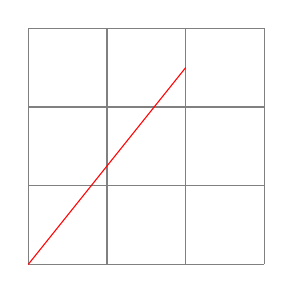
\begin{tikzpicture}
    \draw[gray] grid (3,3);
    \draw[red] (0,0) -- (2,2.5);
\end{tikzpicture}

\vspace{1cm}

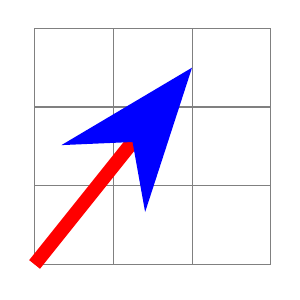
\begin{tikzpicture}
    \draw[gray] grid (3,3);
    \draw[red,-{Stealth[scale=2,color=blue]},line width=5pt] (0,0) -- (2,2.5);
\end{tikzpicture}

\vspace{1cm}

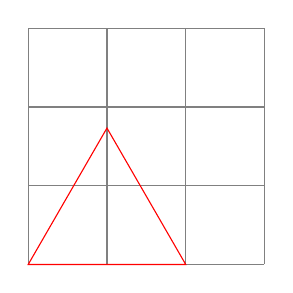
\begin{tikzpicture}
    \draw[gray] grid (3,3);
    \draw[color=red] (0,0) -- (60:2) -- (2,0) -- cycle;
\end{tikzpicture}

\vspace{1cm}

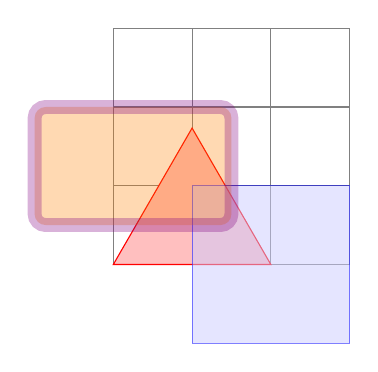
\begin{tikzpicture}
    \draw[gray] grid (3,3);
    \draw[color=red,fill=pink] (0,0) -- (60:2) -- (2,0) -- cycle;
    \draw[color=blue,fill=blue!20,opacity=0.5] (1,-1) -- (1,1) -- (3,1) -- (3,-1) -- cycle;
    \draw[fill=orange, opacity=0.3,rounded corners,line width=5pt,draw=violet] (-1,0.5) rectangle (1.5,2);
\end{tikzpicture}

\clearpage
\section{Basic Nodes}
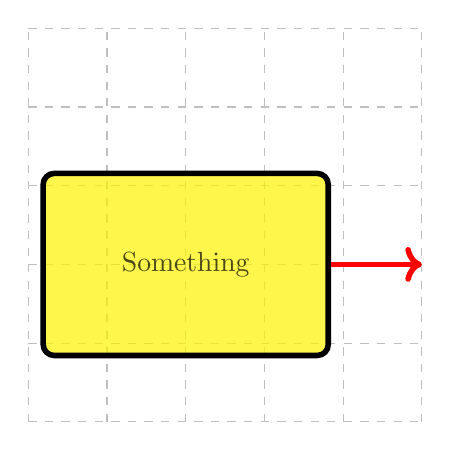
\begin{tikzpicture}
    \draw[gray!50,dashed] grid (5,5); 
    \node[color=black,fill=yellow, draw,inner sep=1cm, fill opacity=0.7, line width=2pt,rounded corners] (a) at (2,2) {Something};
    \coordinate (coord) at (5,2);
    \draw[red,->,line width=2pt] (a.east) -- (coord); 
\end{tikzpicture}

\vspace{10pt}

\begin{tikzpicture}
    \draw[gray!50,dashed,step=5mm] grid (6,6); 
    \node[] (a) at (3,3){\includegraphics[width=4cm]{images/blue.jpg}};
    \draw[red,->,line width=2pt] ($(a.west) - (2,0)$) -- (a.west);
    \draw[orange,-Stealth, line width=3pt] (0,0) to[out=-40, in=180] (a.center);
\end{tikzpicture}

\end{document}